\chapter{Solution}
\label{solution}
Solution...{\color{red} TODO }
The development phase of addie model

\begin{enumerate}
\item Create a Sample (see on kliendile, testiks ja prototüübiks)
\item Develop the course Materials (peab teadma activities + tagasiside review)
\item Conduct a Run-through (real-time rehearsal testi sõbra peal kogu kursust +  feedback assessment + saab reaalselt teada aja, mis kulub kursuse läbimisele
\end{enumerate}


The implementation phase of the ADDIE Model contains three sub-phases

\begin{enumerate}
\item Train the Instructor
\item Prepare the Learners
\item Arrange the Learning Space
\end{enumerate}

Train the Instructor - course developer is often a trainer too but some cases you need more people to train




\section{Implementation of the e-course}

\subsection{Developing the learning material}
\subsection{Text based learning material}
\subsection{Audio/Visual learning material}
\subsection{Interactive learning material}
\subsection{Online tests and laboratory scenarios}
\subsection{Learning objectives}
\subsection{Technical implementation of the e-course}

\subsubsection{The Environment of Distance Study}
\label{The Environment of Distance Study}
The Environment of Distance Study...

TODO pilt virtuaalaborite süsteemi kontekstist
\subsubsection{Random tags}
\begin{itemize}
	\item normal traffic generator
	\item malicious traffic generator
	\item availability monitor (for grading)
\end{itemize}

\subsubsection{Virtualization Layer}
Siin libvirdist
\subsubsection{Web Application Layer}
Siin Ruby on Rails raamistikust ja veebirakendusest
\subsubsection{Architecture of Distance Laboratory}
Siin räägin üldisest disainist ja allsüsteemidest
\
\begin{figure}[ht]
\centering
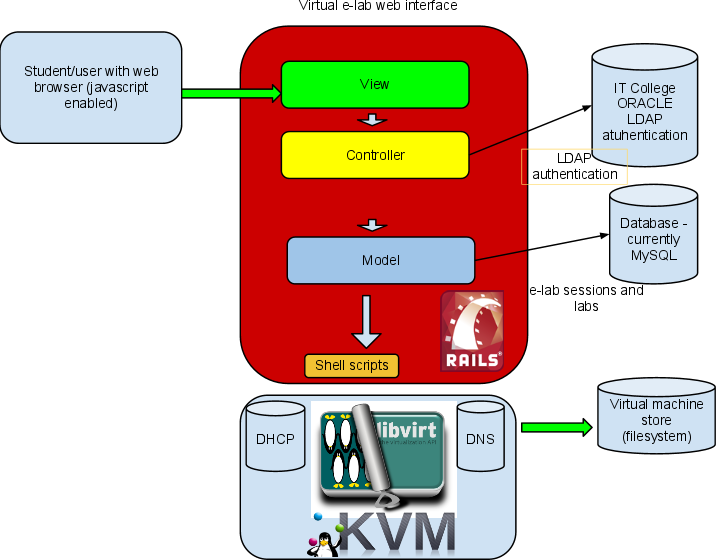
\includegraphics[width=0.8\textwidth]{architecture.png}
\caption{Architecture of Distance Laboratory}
\label{fig:Architecture of Distance Laboratory}
\end{figure}
\

\subsubsection{Security Aspects of Distance Laboratory}

\subsection{Testing the e-course}
\section{Piloting the course}
\subsection{Organizational role}
\subsection{Social role}
\subsection{Pedagogical role}